\documentclass[conference]{IEEEtran}
\IEEEoverridecommandlockouts
\usepackage{cite}
\usepackage{amsmath,amssymb,amsthm}
\usepackage{booktabs}
\usepackage{graphicx}
\usepackage{xcolor}
\usepackage{colortbl}
\usepackage{algorithm}
\usepackage{algpseudocode}
\usepackage{tikz}
\usetikzlibrary{positioning,shapes.geometric,arrows.meta,fit,calc,backgrounds,patterns}
\usepackage{pgfplots}
\usepgfplotslibrary{polar}
\pgfplotsset{compat=1.16}
\usepackage[hidelinks]{hyperref}
\newtheorem{proposition}{Proposition}

% Set to \extendedtrue after the extra questions have been run and Table~\ref{tab:extended} is filled in.
\newif\ifextended
\extendedfalse

\begin{document}

\title{Agreement-Gated Visual Adjudication for\\Long Visual Document Question Answering}

\author{\IEEEauthorblockN{Mariam Zahid}
\IEEEauthorblockA{\textit{Artificial Intelligence, Fast NUCES}\\
Islamabad, Pakistan}}

\maketitle

\begin{abstract}
Long visual document question answering systems first find the evidence pages, then sample several candidate answers, and finally let an Adjudicator choose one. In DocLens, this last step runs on every question and reads only the text of the candidates, although the sampled answers already agree on about half of the questions. We study when adjudication is needed and what the Adjudicator should see. We propose gated visual adjudication. An agreement gate skips the Adjudicator when all $k$ sampled answers agree, and otherwise a visual Adjudicator checks the candidates against the evidence pages. We formalize the pipeline, derive the accuracy change and the token cost of the gate, and show when a gate is lossless. With Qwen3-VL-8B on 200 MMLongBench-Doc questions, the method calls the Adjudicator on 52\% of the questions instead of all of them and raises the accuracy from 56.3\% to 57.3\%, with gains on table (+5.0) and figure (+2.0) questions, at 6.7\% more tokens. The improvement lies within the sampling error of 200 questions. The agreement of the samples predicts when adjudication helps, and most remaining errors come from evidence retrieval and reading, not from the final decision.
\end{abstract}

\begin{IEEEkeywords}
document question answering, long documents, multi-agent systems, adjudication, agreement gate, vision-language models
\end{IEEEkeywords}

% Paper body shared by main.tex (IEEEtran) and sn-article.tex (Springer Nature).
% Needs, from the wrapper: \ifextended, the proposition environment, the algorithm packages, colortbl, pgfplots (with the polar library).

\section{Introduction}
\label{sec:intro}

Visual document understanding (VDU) is the task of reading a document the way a person does and turning what is read into useful information. A document is more than a string of words: it carries tables, charts, figures, icons and a page layout, and a VDU system has to interpret all of these signals together \cite{huang2022layoutlmv3,kim2022donut}. Much of VDU is posed as question answering. In visual question answering (VQA), a model receives an image and a natural-language question and returns an answer. When the image is a document page, the task becomes document VQA (DocVQA) \cite{mathew2021docvqa}, and closely related variants ask questions about charts \cite{masry2022chartqa}, infographics \cite{mathew2022infographicvqa} and slide decks \cite{tanaka2023slidevqa}. Questions of this kind were first asked about single pages, but the documents that people actually read are long. Annual reports, academic papers and technical manuals run to dozens of pages, and the evidence for one question may be a table on one page and a chart on another \cite{tito2023mpdocvqa,vanlandeghem2023dude}.

The ability to answer such questions reliably is important because long documents hold a large share of human knowledge in finance, science and engineering, and small misreadings can turn into costly decisions. An analyst who extracts a wrong figure from an earnings report, an engineer who follows a wrong step from a specification, or an educator who prepares material from a misread paper can spread the error further \cite{slideagent}. Long visual documents are formidably difficult even for strong vision-language models (VLMs), because the evidence is spread over many pages and mixes text with visual elements, and because a model that fails to find the evidence tends to invent an answer instead of admitting that the document does not contain one \cite{zhu2025doclens,ma2024mmlongbench}. A useful system therefore has to be accurate and also honest about what the document supports.

These properties make long-document VQA relevant to many practical settings, including financial analysis, scientific literature assistants, technical support over product manuals, and the search of legal and administrative archives. Real inputs are often imperfect: scanned books contain recognition noise that even modern language models do not remove \cite{nguyen2025gec}, and historical pages need restoration before text can be read \cite{guan2025preocr}. These conditions show that a document system is judged on realistic input and not on clean renderings only. They also show that the quality of the evidence handed to the final answer step cannot be taken for granted.

Research on this problem has moved quickly through three stages. Early pipelines ran optical character recognition (OCR) and fed the words and their positions to a language model, which loses fine layout cues and passes recognition errors down the pipeline \cite{huang2022layoutlmv3}. OCR-free models then read the page image directly \cite{kim2022donut}, and today's VLMs accept several page images at once. For long documents, however, feeding all pages to one model scales poorly because of the cost of attention over long inputs and the tendency of models to overlook content in the middle of a long context \cite{ma2024mmlongbench,deng2025longdocurl}. Retrieval-based systems reduce this cost by selecting a few pages before answering \cite{santhanam2022colbertv2,faysse2024colpali,yu2024visrag,tanaka2025vdocrag}, yet they suffer from retrieval errors: on MMLongBench-Doc, Gemini-2.5-Pro recalls only 68\% of the evidence pages, and ColBERT and ColPali reach a Recall@10 of only 55.3\% \cite{zhu2025doclens}. Even on the right page, a detail inside a chart or a table can be lost in a full-page view, much like reading a map without a magnifying glass \cite{zhu2025doclens,slideagent}.

The most recent work therefore divides the task between several agents. SlideAgent builds hierarchical knowledge at the document, page and element levels and surpasses its backbone models by 7.9\% and 9.8\% for proprietary and open-source models, respectively \cite{slideagent}. Doc-V* treats document VQA as sequential evidence gathering, starting from a thumbnail overview and then fetching pages actively, and it improves out-of-domain accuracy by up to 47.9\% over a retrieval baseline after training with imitation and reinforcement learning \cite{docvstar}. ORCA decomposes a query into reasoning steps, routes each step to a specialized agent and refines the answer iteratively \cite{orca}. SimpleDoc retrieves pages and refines the query over several rounds \cite{jain2025simpledoc}. DocLens, which is directly related to our work, adds a Lens Module with a Page Navigator and an Element Localizer that reach near-perfect evidence recall and crop the relevant tables and figures. Its Reasoning Module then follows a sampling-adjudication process: an Answer Sampler proposes several candidate answers, and an Adjudicator selects the final one \cite{zhu2025doclens}. This design reaches the best published results on MMLongBench-Doc and, for the first time, surpasses human experts on parts of it \cite{zhu2025doclens}. Its sampling-adjudication step follows the idea of combining several reasoning paths \cite{wang2023selfconsistency,wei2022cot} and of asking a language model to judge candidate answers \cite{zheng2023judging}.

The research problem we study begins after the evidence has been found. Once a sampling-based document agent holds several candidate answers, it must decide which one to return, and each design choice at this step affects both the accuracy and the cost of the system. In DocLens, the Adjudicator runs on every question and reads only the text of the candidate analyses, never the document pages. Its own ablation shows that the whole Reasoning Module adds only 0.6 points for Gemini-2.5-Pro (67.0 without it and 67.6 with it) \cite{zhu2025doclens}, which raises two questions that no existing document agent answers: when does the final decision step add value, and what should the decision maker be shown?

The literature points to a gap here. SlideAgent, Doc-V* and DocLens all commit to an answer on every query \cite{slideagent,docvstar,zhu2025doclens}, and evidence from ORCA suggests that this is not harmless: 12\% of its analyzed failures are over-refinement, where a verification stage overrides an answer that was already correct, and ORCA skips its debate stages when two agents agree, which happens in 77\% of its cases \cite{orca}. Revising an answer without new information is known to hurt in language models \cite{huang2024selfcorrect}, while the agreement between sampled answers is a known signal of uncertainty and hallucination \cite{kuhn2023semantic,manakul2023selfcheckgpt}, and adjusting verbal uncertainty at inference time reduces confident hallucinations in short-form question answering by about 30\% \cite{ji2025verbal}. Cascades that call an expensive model only when needed are likewise a proven way to save cost \cite{chen2024frugalgpt}. Yet this line of work has been developed for text-only language models, and no study has used the agreement of sampled answers to decide when a document agent needs an adjudicator, or has given that adjudicator the pages. Our reproduction of DocLens with Qwen3-VL-8B motivates this question: the eight sampled answers agree on 48\% of the questions, the text-only Adjudicator and the majority vote score differently on only 4.5\% of the questions, and still for 15.5\% of the questions a correct candidate exists but the final answer is wrong.

To address this gap, we propose gated visual adjudication. An agreement gate counts how many of the $k=8$ sampled answers agree and returns the majority answer without further processing when all of them agree. When they disagree, a visual Adjudicator reads the evidence pages together with the candidate analyses and answers, and chooses one of the candidates or abstains. The method requires no training and leaves the DocLens prompts for the Lens Module and the Answer Sampler unchanged. With Qwen3-VL-8B on 200 MMLongBench-Doc questions, it calls the Adjudicator on 52\% of the questions instead of all of them and raises the accuracy from 56.3\% to 57.3\%, with the largest gains on table and figure questions, at the price of 6.7\% more tokens; the gain is small, and we report its confidence interval. Our contributions are as follows. We give a formal treatment of the decision step of sampling-based document agents, with closed-form expressions for the accuracy change and the token cost of an agreement gate and a condition under which a gate is lossless. We introduce a unanimity-gated visual Adjudicator that conditions on the retrieved evidence without extra parameters or training. We present a controlled evaluation on MMLongBench-Doc with Qwen3-VL-8B, covering reproductions of the vanilla, OCR and DocLens baselines, an analysis of accuracy by sample agreement, a candidate-ceiling and error-source analysis, and paired-bootstrap confidence intervals. The remainder of this paper is organized as follows. Section~\ref{sec:formulation} formalizes the problem, Section~\ref{sec:method} presents the method, Section~\ref{sec:experiments} reports the experiments, Section~\ref{sec:analysis} analyzes the results, Section~\ref{sec:related} reviews related work, and Section~\ref{sec:conclusion} concludes.

\section{Problem Formulation}
\label{sec:formulation}

We study question answering over long visual documents. A document is a sequence of pages $D=(p_1,\dots,p_N)$, where each page $p_j$ is a screenshot. From each page we obtain its text $t_j$ and a set of visual elements $V_j$ such as tables, figures and charts. Given a question $q$, the goal is to return an answer $\hat y$ that matches the reference answer $y^\ast$. Following DocLens \cite{zhu2025doclens}, we factor the answering function into evidence extraction, answer sampling and a final decision. The Lens Module $\mathcal{L}$ extracts the evidence
\begin{equation}
E=\mathcal{L}(D,q)=\{(p_j,t_j,V_j)\}_{j\in P},\qquad P\subseteq\{1,\dots,N\},
\label{eq:lens}
\end{equation}
where $P$ is the set of pages found by the Page Navigator. The Answer Sampler draws $k$ reasoning--answer pairs from the backbone $\pi_\theta$ at temperature $T$,
\begin{equation}
(r_i,y_i)\sim\pi_\theta(\,\cdot\mid q,E\,),\qquad i=1,\dots,k.
\label{eq:sampler}
\end{equation}
A final decision function $\Phi$ maps the question, the evidence and the candidates to the answer,
\begin{equation}
\hat y=\Phi\bigl(q,E,\{(r_i,y_i)\}_{i=1}^{k}\bigr).
\label{eq:decision}
\end{equation}
DocLens uses a text-only Adjudicator $\mathcal{A}_{\mathrm{text}}(q,\{(r_i,y_i)\})$ for $\Phi$, which ignores $E$ and runs on every question. Let $s(\hat y,y^\ast)\in[0,1]$ be the official benchmark score, which gives partial credit for list answers. The accuracy of a decision function over $M$ questions is
\begin{equation}
\mathrm{Acc}(\Phi)=\frac{1}{M}\sum_{m=1}^{M}s\bigl(\Phi(q_m,E_m,\{(r_i,y_i)\}_m),\,y^\ast_m\bigr).
\label{eq:acc}
\end{equation}
The cost $C(\Phi)$ is the number of tokens spent per question, summed over all steps. We look for a decision function with high $\mathrm{Acc}(\Phi)$ and low $C(\Phi)$, without training and without changing $\mathcal{L}$ and $\pi_\theta$.

\section{Gated Visual Adjudication}
\label{sec:method}

Figure~\ref{fig:pipeline} shows the pipeline. The Lens Module and the Answer Sampler are those of DocLens. We change only the decision step $\Phi$ of Eq.~\eqref{eq:decision}.

\begin{figure*}[t]
\centering
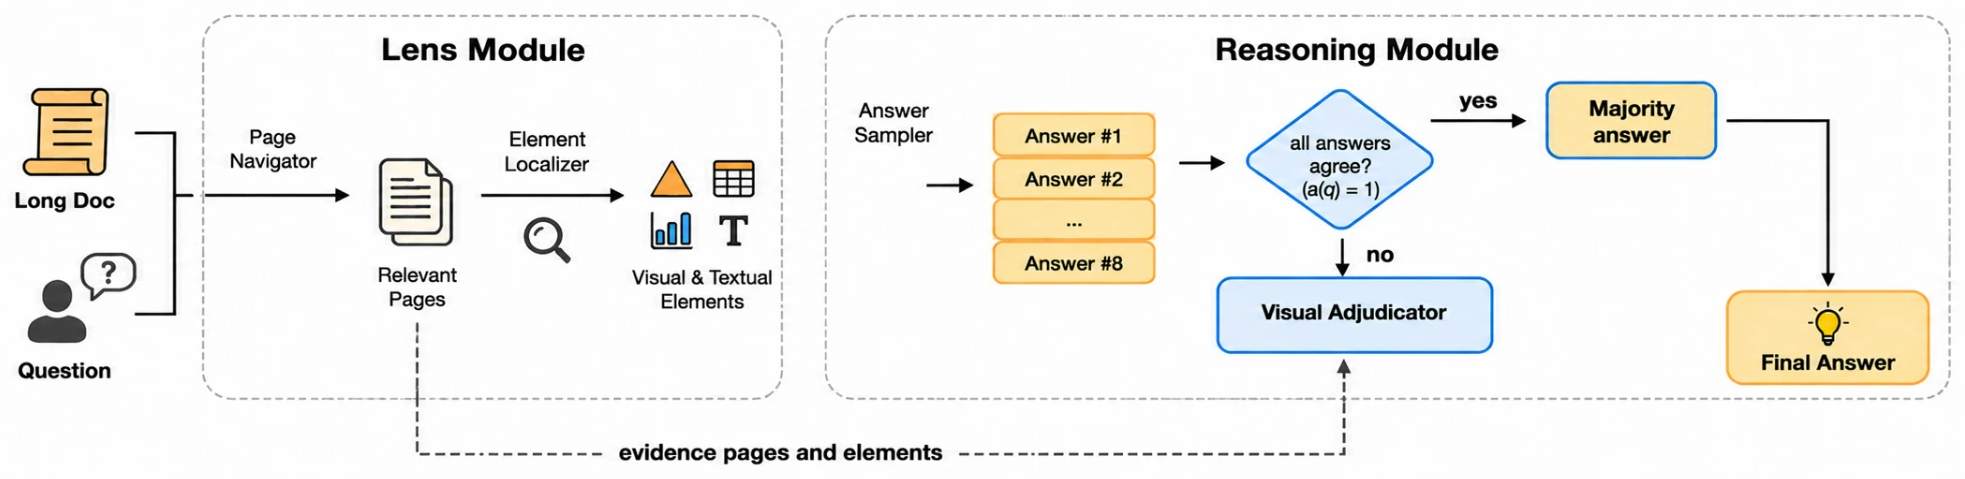
\includegraphics[width=0.96\textwidth]{fig_pipeline.png}
\caption{Overall pipeline of gated visual adjudication. Given a long document and a question, the Lens Module (unchanged from DocLens) retrieves the relevant pages and the visual and textual elements on them. The Answer Sampler draws $k=8$ candidate answers. The agreement gate returns the majority answer when all candidates agree. Otherwise the Visual Adjudicator reads the evidence pages and elements together with the candidates and selects the final answer. Blue outlines mark our additions.}
\label{fig:pipeline}
\end{figure*}

\subsection{Agreement Gate}
Let $n(\cdot)$ be a normalization that lower-cases an answer and removes spaces and punctuation. Let $V=\{i: n(y_i)\notin\{\emptyset,\text{error}\}\}$ be the valid candidates, and let $m_c=|\{i\in V:n(y_i)=c\}|$ count the candidates that equal the normalized answer $c$. The majority answer and the agreement of the question are
\begin{equation}
\hat y_{\mathrm{maj}}=\arg\max_c m_c,\qquad a(q)=\frac{\max_c m_c}{|V|}\in\Bigl[\tfrac{1}{|V|},1\Bigr],
\label{eq:agreement}
\end{equation}
with $a(q)=0$ when $V=\emptyset$. The gate returns the majority answer when the agreement reaches a threshold $\tau$ and calls an adjudicator otherwise:
\begin{equation}
\Phi_\tau(q)=
\begin{cases}
\hat y_{\mathrm{maj}} & \text{if } a(q)\ge\tau,\\[2pt]
\mathcal{A}\bigl(q,E,\{(r_i,y_i)\}_{i=1}^{k}\bigr) & \text{otherwise.}
\end{cases}
\label{eq:gate}
\end{equation}
In our main setting $\tau=1$, so the adjudicator is skipped only when all valid candidates agree. This rule is fixed in advance and has no tuned parameter. The agreement $a(q)$ is the same kind of signal as the consistency of sampled answers that is used to estimate uncertainty and to detect hallucinations \cite{kuhn2023semantic,manakul2023selfcheckgpt}, and the gate is a reject option in the sense of selective prediction \cite{jiang2021calibration}: the pipeline abstains from the expensive step when its confidence is high.

\subsection{Visual Adjudicator}
The text-only Adjudicator of DocLens decides from the written analyses alone. Our visual Adjudicator $\mathcal{A}_{\mathrm{vis}}$ also receives the evidence $E$, which consists of the page screenshots, the cropped elements and the page text that the Answer Sampler saw:
\begin{equation}
\hat y=\mathcal{A}_{\mathrm{vis}}\bigl(q,E,\{(r_i,y_i)\}_{i=1}^{k}\bigr)\in\{y_1,\dots,y_k\}\cup\{\bot\},
\label{eq:visual}
\end{equation}
where $\bot$ stands for the answer ``Not answerable''. The visual Adjudicator uses the same backbone, so there are no new parameters. Its prompt is the DocLens Adjudicator prompt with two additions. The model must check the values that the competing answers depend on against the page images, and it must choose the text of one candidate instead of writing a new answer, or answer ``Not answerable'' when the pages do not contain the requested value. Each analysis is cut to 2,000 characters, the temperature is 0, and if the output cannot be parsed we return the DocLens answer. This design follows the idea of using a language model as a judge \cite{zheng2023judging}, with the difference that the judge sees the evidence. Algorithm~\ref{alg:gva} gives the complete procedure.

\begin{algorithm}[t]
\caption{Gated visual adjudication for one question}
\label{alg:gva}
\begin{algorithmic}[1]
\Require document $D$, question $q$, samples $k$, threshold $\tau$
\State $E\gets\mathcal{L}(D,q)$ \Comment{Lens Module}
\State draw $(r_i,y_i)\sim\pi_\theta(\cdot\mid q,E)$, $i=1,\dots,k$ \Comment{sampler}
\State compute $V$, $\hat y_{\mathrm{maj}}$ and $a(q)$ by Eq.~\eqref{eq:agreement}
\If{$a(q)\ge\tau$}
  \State \Return $\hat y_{\mathrm{maj}}$ \Comment{no call}
\Else
  \State \Return $\mathcal{A}_{\mathrm{vis}}(q,E,\{(r_i,y_i)\}_{i=1}^{k})$
\EndIf
\end{algorithmic}
\end{algorithm}

\subsection{Accuracy and Cost of the Gate}
Let $G_\tau=\{q: a(q)\ge\tau\}$ be the questions that the gate answers itself and $p=\Pr[q\in G_\tau]$ the skipped fraction. Let $\Phi_{\mathcal{A}}$ be the pipeline that always runs the adjudicator $\mathcal{A}$.

\begin{proposition}
\label{prop:acc}
For the same adjudicator $\mathcal{A}$,
\[
\mathrm{Acc}(\Phi_\tau)-\mathrm{Acc}(\Phi_{\mathcal{A}})=\frac{1}{M}\sum_{q\in G_\tau}\Bigl[s(\hat y_{\mathrm{maj}},y^\ast)-s\bigl(\mathcal{A}(q),y^\ast\bigr)\Bigr].
\]
\end{proposition}
\begin{proof}
The two pipelines return the same answer for every question outside $G_\tau$, so only the questions in $G_\tau$ contribute to the difference.
\end{proof}

The difference is the number of over-corrections avoided minus the number of fixes lost on $G_\tau$. For $\tau=1$ and the text-only Adjudicator, it is zero whenever the Adjudicator returns the shared answer on unanimous questions, and we measure exactly this in Section~\ref{sec:analysis}.

\begin{proposition}
\label{prop:cost}
Let $C_0$ be the tokens spent by $\mathcal{L}$ and the sampler, and $C_{\mathcal{A}}$ the tokens of one adjudicator call. The expected cost is $C(\Phi_\tau)=C_0+(1-p)\,C_{\mathcal{A}}$, so the gate saves $p\,C_{\mathcal{A}}$ per question. Compared with always running the text-only Adjudicator (cost $C_{\mathrm{text}}$), a visual Adjudicator (cost $C_{\mathrm{vis}}$) behind the gate does not increase the cost if and only if $p\ge 1-C_{\mathrm{text}}/C_{\mathrm{vis}}$.
\end{proposition}
\begin{proof}
The adjudicator is called with probability $1-p$, which gives the expected cost. The condition follows from $(1-p)C_{\mathrm{vis}}\le C_{\mathrm{text}}$.
\end{proof}

Two bounds limit what any selection among the candidates can do. No decision function that only selects among the candidates can exceed $\mathrm{pass@}k=\frac{1}{M}\sum_m\max_i s(y_i,y^\ast_m)$, and a gate over $\hat y_{\mathrm{maj}}$ and $\mathcal{A}_{\mathrm{text}}$ cannot exceed the oracle that picks the better of the two answers for each question.

\section{Experiments}
\label{sec:experiments}

In this section, we first describe the experimental setup (Section~\ref{sec:setup}), including the benchmark, the metrics, the models and the baselines. We then present the main results (Section~\ref{sec:main}).

\subsection{Experimental Setup}
\label{sec:setup}
\textbf{Benchmark and Metrics.} We use MMLongBench-Doc \cite{ma2024mmlongbench}, which has 1,082 questions on long PDF documents of 49.4 pages on average. Each question has an evidence source (plain text, layout, chart, table or figure), and 22.8\% of the questions have no answer in the document, which makes it possible to measure hallucination. Human experts reach 65.8\% on this benchmark. The original DocLens evaluation of Qwen3-VL-8B uses a random sample of 200 questions that is not published \cite{zhu2025doclens}, so we draw our own sample of 200 questions with a fixed seed. It covers 95 documents and is the same for every method. We follow the official rule-based scoring, which compares the extracted answer with the reference and gives partial credit for lists. We report accuracy (Eq.~\eqref{eq:acc}) and four further measures. The Adjudicator rate is $\frac{1}{M}\sum_m\mathbb{1}[a(q_m)<\tau]$. With $\hat y_m$ the returned answer and a score of at least 0.5 counted as correct, the over-correction rate and the fix rate are
\begin{equation}
\begin{aligned}
\mathrm{OC}&=\tfrac{1}{M}\textstyle\sum_m\mathbb{1}\bigl[s(\hat y_{\mathrm{maj},m},y^\ast_m)\ge0.5,\; s(\hat y_m,y^\ast_m)<0.5\bigr],\\
\mathrm{Fix}&=\tfrac{1}{M}\textstyle\sum_m\mathbb{1}\bigl[s(\hat y_{\mathrm{maj},m},y^\ast_m)<0.5,\; s(\hat y_m,y^\ast_m)\ge0.5\bigr],
\end{aligned}
\label{eq:ocfix}
\end{equation}
so that Proposition~\ref{prop:acc} states that gating changes the accuracy by the difference of the two rates on the skipped questions. The fourth measure is the number of tokens per question. For the difference $\Delta=\mathrm{Acc}(\Phi_1)-\mathrm{Acc}(\Phi_2)$ of two methods, we resample the $M$ questions with replacement 10,000 times, recompute $\Delta$ on each resample, and report the 2.5th and 97.5th percentiles as the 95\% confidence interval.

\textbf{Models and Baselines.} All methods use Qwen3-VL-8B-Instruct.\footnote{\url{https://huggingface.co/Qwen/Qwen3-VL-8B-Instruct}} We compare vanilla Qwen3-VL-8B with page screenshots only, Qwen3-VL-8B with OCR text added to each page, DocLens, majority voting over the eight samples, the gate with the text-only Adjudicator (with $\tau=1$ and with a threshold chosen by five-fold cross-validation over documents), and our gated visual Adjudicator. For context, Table~\ref{tab:main} also lists published results of other methods and backbones, which were evaluated on the full benchmark or on other samples.

\textbf{Implementation Details.} We serve the model with vLLM \cite{kwon2023vllm} on two NVIDIA T4 GPUs with tensor parallelism 2. We use the DocLens settings ($k=8$ samples at $T=0.7$, eight Page Navigator samples) and extract the page text with MinerU\footnote{\url{https://github.com/opendatalab/MinerU}}. The memory of the T4 GPUs limits the context to 40,960 tokens. The Page Navigator therefore reads documents in chunks of six pages, images are halved when a prompt is too long, and answers are extracted for scoring with the same Qwen model instead of Gemini-2.5-Flash. These choices explain part of the gap to the published numbers.

\subsection{Main Results}
\label{sec:main}
Table~\ref{tab:main} presents the main results. Our baselines are close to the published Qwen3-VL-8B numbers for vanilla prompting (40.9 against 43.0) and lower for OCR (37.3 against 42.9) and for DocLens (56.3 against 61.1). Three causes are likely: the shorter context of the T4 setup, the Qwen answer extractor, and a lower page recall of our Page Navigator (88.4\% against 97.3\% for Gemini-2.5-Pro in the DocLens paper). OCR text hurts in our setup, while the original paper reports almost equal values, which we attribute to the longer prompts that OCR text creates. DocLens is clearly better than both baselines, most of all on unanswerable questions (75.7 against 45.0 for vanilla).

\begin{table*}[t]
\caption{Main results on MMLongBench-Doc. We report accuracy (\%) for five evidence sources: plain text (TXT), layout (LAY), chart (CHA), table (TAB) and figure (FIG), for unanswerable questions (UNA) and for all questions (ALL). $^\dagger$ marks results taken from the original paper, so some cells are unavailable; the other published values, including those of Gemini-2.5, MACT, M3DocRAG and MDocAgent, are quoted from the DocLens paper \cite{zhu2025doclens}. $^\ddagger$ marks results on a random sample of 200 questions (our own sample for our runs). Bold marks the best value per column within the Qwen3-VL-8B block of our runs. Backbones and samples differ across blocks, so only the Qwen3-VL-8B rows are directly comparable. Human experts reach 65.8.}
\label{tab:main}
\centering
\footnotesize
\setlength{\tabcolsep}{4.5pt}
\begin{tabular}{@{}lccccccc@{}}
\toprule
Model & TXT & LAY & CHA & TAB & FIG & UNA & ALL \\
\midrule
\multicolumn{8}{c}{\textit{Vanilla VLMs}} \\
GPT-4o$^\dagger$ \cite{ma2024mmlongbench} & 46.3 & 46.0 & 45.3 & 50.0 & 44.1 & 20.2 & 42.8 \\
Claude-4-Sonnet & 50.4 & 49.4 & 50.5 & 57.3 & 43.9 & 59.0 & 53.4 \\
Gemini-2.5-Flash & 44.0 & 53.2 & 46.0 & 43.9 & 48.2 & 56.7 & 49.6 \\
Gemini-2.5-Pro & 52.1 & 62.1 & 55.5 & 55.3 & 54.0 & 59.9 & 58.1 \\
\midrule
\multicolumn{8}{c}{\textit{VLMs augmented with OCR}} \\
Gemini-2.5-Flash & 55.9 & 54.9 & 52.7 & 63.4 & 50.3 & 60.8 & 58.5 \\
Gemini-2.5-Pro & 59.7 & 65.3 & 60.8 & 68.3 & 55.7 & 58.4 & 63.3 \\
\midrule
\multicolumn{8}{c}{\textit{VLM-based agentic frameworks}} \\
MACT (MiMo-VL-7B)$^\dagger$ & -- & -- & -- & -- & -- & -- & 47.4 \\
M3DocRAG (Qwen2-VL-7B)$^\dagger$ & 30.0 & 23.5 & 18.9 & 20.1 & 20.8 & 5.8 & 21.0 \\
MDocAgent (GPT-4o)$^\dagger$ & -- & -- & -- & -- & -- & -- & 42.0 \\
Doc-V* (Qwen2.5-VL-7B)$^\dagger$ \cite{docvstar} & -- & -- & -- & -- & -- & -- & 42.1 \\
SimpleDoc (Claude-4-Sonnet) \cite{jain2025simpledoc} & 52.1 & 53.3 & 58.3 & 62.4 & 46.9 & 66.5 & 58.6 \\
DocLens (Gemini-2.5-Pro) \cite{zhu2025doclens} & 63.7 & 64.6 & 64.3 & 69.7 & 60.2 & 72.2 & 67.6 \\
\midrule
\multicolumn{8}{c}{\textit{Qwen3-VL-8B, published$^{\dagger\ddagger}$}} \\
Vanilla & -- & -- & -- & -- & -- & -- & 43.0 \\
Screenshots + OCR & -- & -- & -- & -- & -- & -- & 42.9 \\
DocLens & -- & -- & -- & -- & -- & -- & 61.1 \\
\midrule
\multicolumn{8}{c}{\textit{Qwen3-VL-8B, our runs$^\ddagger$}} \\
Vanilla & 38.1 & 47.3 & 30.3 & 36.7 & 47.5 & 45.0 & 40.9 \\
Screenshots + OCR & 32.8 & 24.0 & 20.8 & 27.3 & 38.1 & 56.8 & 37.3 \\
DocLens (our reproduction) & \textbf{51.2} & \textbf{48.0} & \textbf{41.5} & 44.8 & 53.7 & \textbf{75.7} & 56.3 \\
\rowcolor{black!8}
Gated visual adjudication (ours) & \textbf{51.2} & \textbf{48.0} & \textbf{41.5} & \textbf{49.8} & \textbf{55.7} & 73.0 & \textbf{57.3} \\
\bottomrule
\end{tabular}
\end{table*}

On the controlled comparison of our runs, majority voting without any Adjudicator is 1.5 points below DocLens. The gate with $\tau=1$ and the text-only Adjudicator keeps the accuracy of DocLens (56.3) and removes 48\% of the Adjudicator calls. Our gated visual Adjudicator reaches 57.3, which is 1.0 point above DocLens and 2.5 points above majority voting. The 95\% confidence interval of the gain over DocLens is $-2.5$ to $+4.5$ points, and the interval of the gain over majority voting is $-0.5$ to $+5.9$ points, so a sample of 200 questions cannot separate the methods. On the 104 questions where the answers disagree, the accuracy rises from 36.9 to 38.8: the visual Adjudicator fixes 7 questions that DocLens answers wrongly and breaks 5 that DocLens answers correctly.

The gain is concentrated where values must be read from the page image. Table~\ref{tab:main} and Fig.~\ref{fig:radar}(a) show gains of +5.0 on table questions and +2.0 on figure questions, and none on text, layout and chart questions. Unanswerable questions lose 2.7 points, because the visual Adjudicator sometimes accepts a value that is close to the requested one. We discuss this in Section~\ref{sec:analysis}.

\begin{figure*}[t]
\centering
\begin{minipage}[t]{0.47\textwidth}
\centering
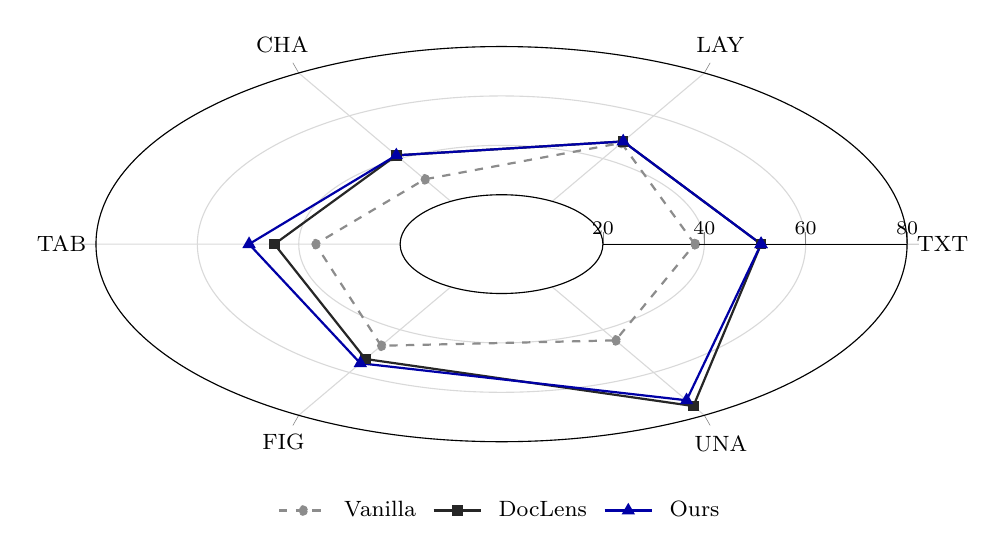
\begin{tikzpicture}
\begin{polaraxis}[
  width=0.98\linewidth, height=6.6cm,
  xtick={0,60,120,180,240,300}, xticklabels={TXT,LAY,CHA,TAB,FIG,UNA},
  ymin=20, ymax=80, ytick={20,40,60,80}, yticklabels={20,40,60,80},
  ticklabel style={font=\footnotesize}, y tick label style={font=\scriptsize},
  grid=both, grid style={black!15},
  legend style={font=\footnotesize, at={(0.5,-0.12)}, anchor=north, legend columns=3, draw=none, column sep=4pt},
  legend cell align=left
]
\addplot[mark=*, mark size=1.5pt, color=black!45, thick, dashed] coordinates {(0,38.1)(60,47.3)(120,30.3)(180,36.7)(240,47.5)(300,45.0)(360,38.1)};
\addplot[mark=square*, mark size=1.5pt, color=black!85, thick] coordinates {(0,51.2)(60,48.0)(120,41.5)(180,44.8)(240,53.7)(300,75.7)(360,51.2)};
\addplot[mark=triangle*, mark size=2pt, color=blue!65!black, thick] coordinates {(0,51.2)(60,48.0)(120,41.5)(180,49.8)(240,55.7)(300,73.0)(360,51.2)};
\legend{Vanilla, DocLens, Ours}
\end{polaraxis}
\end{tikzpicture}

\footnotesize (a) Accuracy by evidence source
\end{minipage}\hfill
\begin{minipage}[t]{0.50\textwidth}
\centering
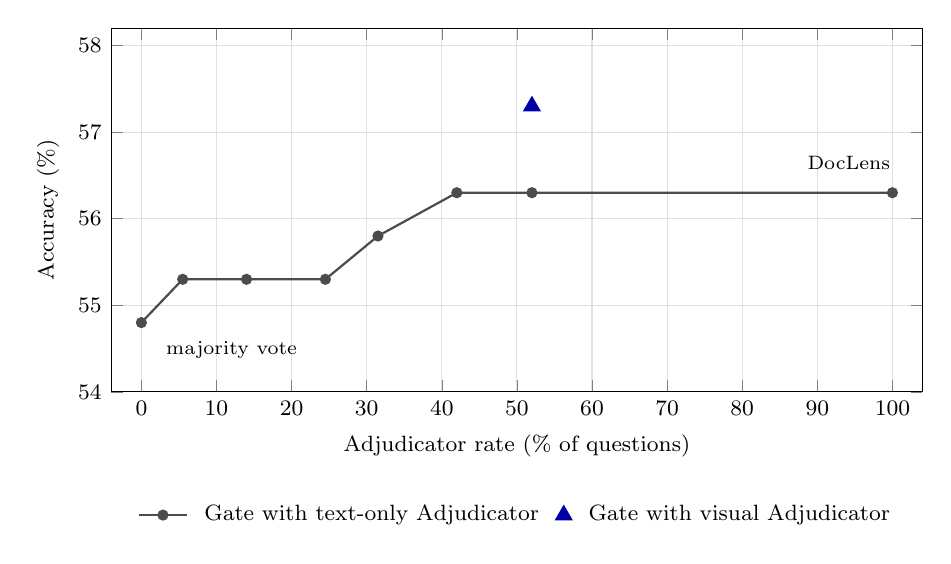
\begin{tikzpicture}
\begin{axis}[
  width=0.98\linewidth, height=6.2cm,
  xlabel={Adjudicator rate (\% of questions)}, ylabel={Accuracy (\%)},
  xmin=-4, xmax=104, ymin=54, ymax=58.2,
  label style={font=\footnotesize}, tick label style={font=\footnotesize},
  legend style={font=\footnotesize, at={(0.5,-0.28)}, anchor=north, legend columns=2, draw=none, column sep=4pt},
  grid=both, grid style={black!12}
]
\addplot[mark=*, mark size=1.6pt, color=black!70, thick] coordinates {(0,54.8)(5.5,55.3)(14,55.3)(24.5,55.3)(31.5,55.8)(42,56.3)(52,56.3)(100,56.3)};
\addplot[only marks, mark=triangle*, mark size=3.4pt, color=blue!65!black] coordinates {(52,57.3)};
\node[font=\scriptsize, anchor=north west] at (axis cs:2,54.7) {majority vote};
\node[font=\scriptsize, anchor=south east] at (axis cs:101,56.45) {DocLens};
\legend{Gate with text-only Adjudicator, Gate with visual Adjudicator}
\end{axis}
\end{tikzpicture}

\footnotesize (b) Accuracy against Adjudicator rate
\end{minipage}
\caption{(a) Accuracy of vanilla Qwen3-VL-8B, DocLens and our method by evidence source on our 200 questions. (b) Accuracy against the share of questions on which an Adjudicator runs, for gates with thresholds $\tau\in\{0,0.375,\dots,1\}$ and the text-only Adjudicator (circles, from majority voting at 0\% to DocLens at 100\%), and for our gated visual Adjudicator at $\tau=1$ (triangle).}
\label{fig:radar}
\end{figure*}

\section{Analysis}
\label{sec:analysis}

This section analyzes the method with Qwen3-VL-8B on our 200 questions. We begin with an ablation of the gate and the Adjudicator (Section~\ref{sec:ablation}). We then study how the agreement of the samples relates to the value of adjudication (Section~\ref{sec:agreement}), look at where the remaining errors come from (Section~\ref{sec:errors}), and finish with an efficiency analysis (Section~\ref{sec:efficiency}).

\subsection{Ablation on the Gate and the Adjudicator}
\label{sec:ablation}
Table~\ref{tab:ablation} ablates the two parts of the method. Removing the Adjudicator and returning the majority answer lowers the accuracy by 1.5 points, on answerable and on unanswerable questions. Adding the gate with $\tau=1$ in front of the text-only Adjudicator leaves every number unchanged, so the gate saves 48\% of the calls for free. Replacing the text-only Adjudicator behind the gate by the visual one raises the accuracy on answerable questions from 51.9 to 53.7, and it lowers the accuracy on unanswerable questions from 75.7 to 73.0. The accuracy gain therefore comes from the visual input, while the gate decides how often it is used. The cross-validated threshold is worse than the fixed rule: it picks 0.875, 0.75, 0.875, 0.375 and 0.875 in the five folds and reaches 54.8 with 30\% of the calls. Values near $\tau=0.875$ also reach 56.3 (Fig.~\ref{fig:radar}b), but they were found on the same questions, so we do not use them.

\begin{table}[t]
\caption{Ablation of the gate and the Adjudicator on our 200 questions. ANS: answerable, UNA: unanswerable. Tokens are per question; relative cost is measured against DocLens.}
\label{tab:ablation}
\centering
\footnotesize
\setlength{\tabcolsep}{3pt}
\begin{tabular}{@{}lccccccc@{}}
\toprule
Setting & Adjud. & Tokens & Cost & ANS & UNA & ALL \\
\midrule
DocLens (text-only, always) & 100\% & 87,620 & 1.00$\times$ & 51.9 & 75.7 & 56.3 \\
\ \ w/o Adjudicator (majority) & 0\% & 84,977 & 0.97$\times$ & 50.7 & 73.0 & 54.8 \\
\ \ + gate $\tau=1$ & 52\% & 86,649 & 0.99$\times$ & 51.9 & 75.7 & 56.3 \\
\ \ + gate $\tau=1$, visual (ours) & 52\% & 93,456 & 1.07$\times$ & \textbf{53.7} & 73.0 & \textbf{57.3} \\
\bottomrule
\end{tabular}
\end{table}

\subsection{Agreement Predicts the Value of Adjudication}
\label{sec:agreement}
\textbf{Agreement is a reliable signal for the gate.} Figure~\ref{fig:agreement}(a) groups the questions by the agreement $a(q)$ of the eight samples. When all samples agree (48.0\% of the questions), the majority answer and the text-only Adjudicator have the same accuracy (77.3\%), so the gate loses nothing there, as Proposition~\ref{prop:acc} predicts. Accuracy falls quickly as agreement falls, from 77.3 to 42.7, 34.3 and 21.2, and the Adjudicator is above the majority answer only on the disagreeing questions, by 2.5, 2.7 and 3.5 points. This is the pattern that a gate needs: the extra step has value only where the candidates disagree.

\textbf{The candidates contain much more than the Adjudicator uses.} The best of the eight candidates is far above both the majority answer and the Adjudicator on the disagreeing questions (71.3, 62.7 and 60.4 in Fig.~\ref{fig:agreement}a). In total, 72.0\% of the questions have at least one correct candidate (pass@8), against 56.3\% for DocLens. A better decision rule could therefore still gain many points, and the visual Adjudicator recovers only a small part of this gap.

\begin{figure*}[t]
\centering
\begin{minipage}[t]{0.49\textwidth}
\centering
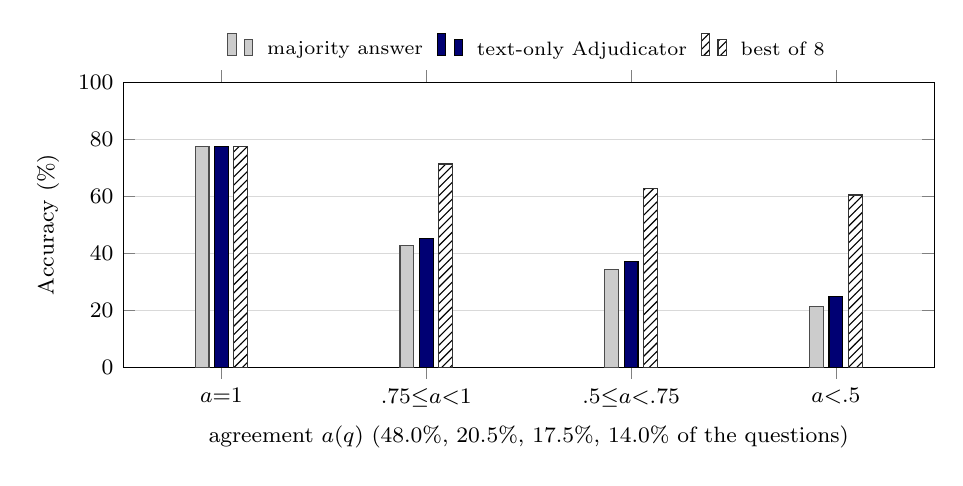
\begin{tikzpicture}
\begin{axis}[
  ybar, bar width=5pt, width=0.98\linewidth, height=5.2cm,
  symbolic x coords={c1,c2,c3,c4},
  xtick=data, xticklabels={$a{=}1$, $.75{\le}a{<}1$, $.5{\le}a{<}.75$, $a{<}.5$},
  ymin=0, ymax=100, enlarge x limits=0.16,
  ylabel={Accuracy (\%)}, ylabel style={font=\footnotesize},
  xlabel={agreement $a(q)$ (48.0\%, 20.5\%, 17.5\%, 14.0\% of the questions)}, xlabel style={font=\footnotesize},
  tick label style={font=\footnotesize},
  legend style={font=\scriptsize, at={(0.5,1.04)}, anchor=south, legend columns=3, draw=none, column sep=3pt},
  ymajorgrids, grid style={black!15}
]
\addplot[fill=black!20, draw=black!70] coordinates {(c1,77.3) (c2,42.7) (c3,34.3) (c4,21.2)};
\addplot[fill=blue!45!black, draw=black] coordinates {(c1,77.3) (c2,45.2) (c3,37.0) (c4,24.7)};
\addplot[fill=white, draw=black!80, postaction={pattern=north east lines}] coordinates {(c1,77.3) (c2,71.3) (c3,62.7) (c4,60.4)};
\legend{majority answer, text-only Adjudicator, best of 8}
\end{axis}
\end{tikzpicture}

\footnotesize (a) Accuracy by agreement level
\end{minipage}\hfill
\begin{minipage}[t]{0.49\textwidth}
\centering
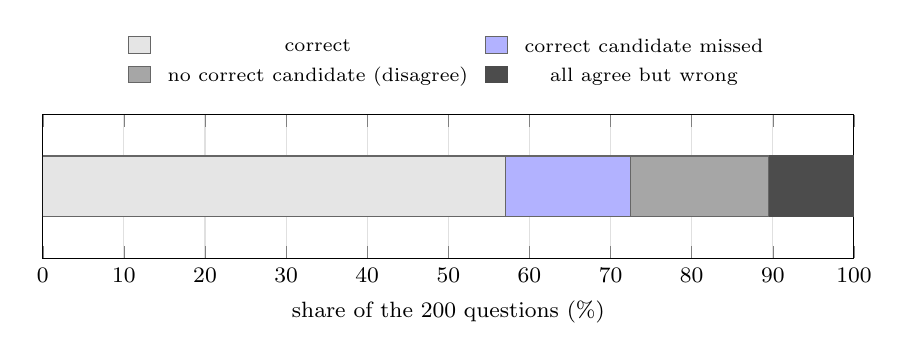
\begin{tikzpicture}
\begin{axis}[
  xbar stacked, bar width=22pt, width=0.98\linewidth, height=3.4cm,
  xmin=0, xmax=100, ytick=\empty, xlabel={share of the 200 questions (\%)}, xlabel style={font=\footnotesize},
  tick label style={font=\footnotesize},
  legend style={font=\scriptsize, at={(0.5,1.12)}, anchor=south, legend columns=2, draw=none, column sep=4pt},
  enlarge y limits=0.6, xmajorgrids, grid style={black!12}
]
\addplot[fill=black!10, draw=black!60] coordinates {(57.0,0)};
\addplot[fill=blue!30, draw=black!60] coordinates {(15.5,0)};
\addplot[fill=black!35, draw=black!60] coordinates {(17.0,0)};
\addplot[fill=black!70, draw=black!70] coordinates {(10.5,0)};
\legend{correct, correct candidate missed, no correct candidate (disagree), all agree but wrong}
\end{axis}
\end{tikzpicture}

\footnotesize (b) Outcome of the 200 questions for DocLens
\end{minipage}
\caption{(a) Accuracy of the majority answer, of the text-only Adjudicator and of the best of the eight candidates (an upper bound) by agreement level. (b) Outcome of the final answer of DocLens, counting a score of at least 0.5 as correct.}
\label{fig:agreement}
\end{figure*}

\subsection{Error Analysis}
\label{sec:errors}
\textbf{Most errors are not decision errors.} Figure~\ref{fig:agreement}(b) splits the outcomes of DocLens. A total of 57.0\% of the questions are answered correctly. Of the 43.0\% that are wrong, 10.5\% have eight identical wrong answers and 17.0\% have disagreeing candidates of which none is correct. These 27.5\% are errors of evidence retrieval or reading that no Adjudicator can repair. The Page Navigator of our run recalls 88.4\% of the evidence pages with a precision of 48.7\% and returns 8.6 pages per question. Only the remaining 15.5\% of the questions have a correct candidate that DocLens does not return, and these are the questions that a better final decision can still win.

\textbf{The visual Adjudicator trades unanswerable accuracy for visual accuracy.} On unanswerable questions, the visual Adjudicator is 2.7 points below DocLens (73.0 against 75.7). When it reads a page that contains a value close to the requested one, it tends to accept the closest candidate instead of answering ``Not answerable''. DocLens already shows that unanswerable questions are the weak point of single-pass VLMs (45.0 for vanilla Qwen3-VL-8B in our runs), so we see an adjudicator that can abstain more reliably as a direct next step.

\subsection{Efficiency Analysis}
\label{sec:efficiency}
Table~\ref{tab:tokens} shows where the tokens go. The Lens Module dominates the cost, the text-only Adjudicator is cheap, and one visual call costs about six times as much as a text-only call. By Proposition~\ref{prop:cost}, the visual Adjudicator is token-neutral only if the gate skips at least $1-C_{\mathrm{text}}/C_{\mathrm{vis}}\approx84\%$ of the questions. Our gate skips 48\%, so the total cost rises by 6.7\% (Table~\ref{tab:ablation}). The gate alone saves only 1.1\% of the tokens, because the text-only Adjudicator is only 3\% of the cost. The method therefore reduces the number of Adjudicator calls, but it does not reduce the total cost. Its value lies in accuracy on visual questions and in the removal of unnecessary calls, not in a lower token bill.

\begin{table}[t]
\caption{Tokens per question by stage for DocLens with Qwen3-VL-8B on our 200 questions. The last line is the cost of one visual Adjudicator call, computed from Table~\ref{tab:ablation}.}
\label{tab:tokens}
\centering
\footnotesize
\begin{tabular}{@{}lcc@{}}
\toprule
Stage & Tokens & Share \\
\midrule
Lens Module & 70,200 & 80.1\% \\
Answer Sampler ($k=8$, one request) & 14,800 & 16.9\% \\
Text-only Adjudicator & 2,600 & 3.0\% \\
\midrule
Visual Adjudicator (one call) & 16,300 & -- \\
\bottomrule
\end{tabular}
\end{table}

\ifextended
\textbf{Additional questions.} We also run DocLens and our method on 400 further questions that do not overlap with the first 200 and were not used to design the method. Table~\ref{tab:extended} shows the result.

\begin{table}[t]
\caption{Accuracy (\%) on additional questions (TBD: to be filled in after the runs).}
\label{tab:extended}
\centering
\footnotesize
\begin{tabular}{@{}lccc@{}}
\toprule
Method & 200 (seed 0) & 400 new & All 600 \\
\midrule
Majority vote & 54.8 & TBD & TBD \\
DocLens & 56.3 & TBD & TBD \\
Gated visual adjudication & 57.3 & TBD & TBD \\
\bottomrule
\end{tabular}
\end{table}
\fi

\section{Related Work}
\label{sec:related}

Reading a long document is not one problem but a chain of them, and the literature on visual document understanding can be read as a history of which link of that chain was repaired first. The first links to be repaired were reading and layout. Early systems ran OCR and fed the words with their positions to a language model, as LayoutLMv3 does with a unified pre-training over text and image patches \cite{huang2022layoutlmv3}, and the benchmarks that measured them asked questions about a single page, such as DocVQA for scanned documents and SlideVQA for slides \cite{mathew2021docvqa,tanaka2023slidevqa}. These pipelines work well on clean pages but pass recognition errors down the chain and break on noisy input, which led to OCR-free models such as Donut that read the page image directly \cite{kim2022donut}. The noise itself has also been attacked upstream. PreP-OCR restores degraded page images and then corrects the recognized text with a ByT5 model, and it lowers the character error rate by 63.9 to 70.3\% on 13,831 historical pages \cite{guan2025preocr}. Correcting text with language models is not free of risk, however. In a study of OCR-scanned German children's books, large language models did not remove the recognition noise effectively, and the authors name overcorrection, where a model changes text that was already right, as an under-analyzed hazard of decoder-based models \cite{nguyen2025gec}. This is a first hint of a theme that returns below: a correction step that always acts can harm an input that did not need it.

The next link to break was length. Real documents have dozens of pages, and benchmarks for this setting, such as MMLongBench-Doc and LongDocURL, show that even strong VLMs fail on them and that many questions cannot be answered from the document at all \cite{ma2024mmlongbench,deng2025longdocurl}. Feeding every page to one model scales poorly in cost and attention, so retrieval-based systems select a few pages first. ColPali scores page images with late interaction, and VisRAG and VDocRAG pass the retrieved page images to a VLM \cite{faysse2024colpali,yu2024visrag,tanaka2025vdocrag}. Retrieval, however, makes errors of its own. On MMLongBench-Doc, ColPali-style retrievers reach a Recall@10 of only 55.3\% and Gemini-2.5-Pro recalls only 68\% of the evidence pages \cite{zhu2025doclens}, and a retrieved page can still hide the cell of a table or the bar of a chart that holds the answer.

These failures moved the field from single models to agents. SimpleDoc retrieves pages with embeddings and page summaries and refines its query over several rounds, which improves accuracy by 3.2\% on average over four DocVQA datasets with fewer retrieved pages \cite{jain2025simpledoc}. SlideAgent builds query-independent knowledge at the document, page and element levels and retrieves from it at inference time \cite{slideagent}. Doc-V* treats the task as active perception: it starts from a thumbnail overview, fetches pages and searches semantically, and it keeps a structured working memory, trained with imitation learning and reinforcement learning \cite{docvstar}. ORCA decomposes a question into reasoning steps, routes them to specialized agents, and then debates and refines the answer, but it is designed and evaluated on single pages \cite{orca}. DocLens, the closest work to ours, finds pages with OCR-augmented VLMs, crops tables and figures with an Element Localizer, and chooses its answer by sampling candidates and letting an Adjudicator pick one \cite{zhu2025doclens}. These systems mostly improve where evidence is found and how agents cooperate. They all commit to an answer on every query, and the step that makes this commitment receives little study.

That step has a long history outside document understanding. Sampling several reasoning paths and taking the most frequent answer is a standard way to reduce errors \cite{wang2023selfconsistency}, and a language model can also act as the judge of candidate answers, although such judges show biases \cite{zheng2023judging}. Yet a model that revises its own answer without outside information can make it worse \cite{huang2024selfcorrect}, and ORCA measures the same effect inside a document agent: 12\% of its analyzed failures are over-refinement, where a later stage overrides an answer that was already correct, and it skips its debate stages when two agents agree, which happens in 77\% of its cases \cite{orca}. The agreement among sampled answers is in turn a reliable signal of uncertainty and hallucination \cite{kuhn2023semantic,manakul2023selfcheckgpt}. Calibrating verbal uncertainty at inference time reduces confident hallucinations by about 30\% in short-form question answering \cite{ji2025verbal}, and cascades call an expensive model only when a cheaper answer is not trusted \cite{chen2024frugalgpt}. All of this work, however, is developed for text-only language models.

Our method sits where these lines of work meet. DocLens adjudicates every question, whereas we skip the Adjudicator when the samples agree. The DocLens Adjudicator reads only the written analyses, whereas ours also reads the evidence pages. And where the agent papers improve evidence finding, we formalize the final decision itself and measure how agreement predicts its value. ORCA also skips stages when its agents agree, but inside a multi-stage pipeline built for single pages, and no earlier work uses the agreement of sampled answers to decide when a long-document agent needs a judge, or shows that judge the pages. The field has learned to find the evidence; our work asks when it can safely stop checking it.

\section{Conclusion}
\label{sec:conclusion}
In this paper, we studied the last step of sampling-based document agents, the choice among candidate answers. We gave a formal view of this step, derived the accuracy and cost of an agreement gate, and proposed a visual Adjudicator that checks the candidates against the evidence pages. With Qwen3-VL-8B on 200 MMLongBench-Doc questions, the gate removes 48\% of the Adjudicator calls without a loss of accuracy, and the visual Adjudicator raises the accuracy from 56.3\% to 57.3\%, with the gain on table and figure questions, at 6.7\% more tokens. The agreement of the samples is a good signal of when adjudication is needed: the Adjudicator never helped on unanimous questions and helped by 2.5 to 3.5 points on the others.

\textbf{Limitations.} The study has several limits. The sample has only 200 questions, so the gain of 1.0 point lies within the sampling error, and we designed the visual Adjudicator after looking at the results on the same questions. Our numbers are below the published ones because of the 2$\times$T4 setup and the Qwen answer extractor. With a stricter extraction prompt, DocLens scores 53.6 and vanilla scores 35.8, and the order of these methods does not change. We did not run the visual Adjudicator on every question, so we cannot separate the effect of the gate from the effect of the visual input in that setting, and we tested one backbone only. Most errors come from evidence retrieval and reading and not from the final decision. Future work is a larger evaluation, other backbones, better page recall, and a visual Adjudicator that can abstain.

\section*{Declarations}
\textit{Data availability.} MMLongBench-Doc is available from its authors \cite{ma2024mmlongbench}. The question sample and the saved answers of all runs are available in the repository below.

\textit{Code availability.} The code and the prompts are available at \url{https://github.com/Mariam1543/aqqal123}.

% Funding, Conflict of interest, Ethics approval and consent, Consent for publication, Materials availability and
% Author contribution: add these statements if the venue asks for them (write ``Not applicable'' where they do not apply).


% Generated by IEEEtran.bst, version: 1.14 (2015/08/26)
\begin{thebibliography}{10}
\providecommand{\url}[1]{#1}
\csname url@samestyle\endcsname
\providecommand{\newblock}{\relax}
\providecommand{\bibinfo}[2]{#2}
\providecommand{\BIBentrySTDinterwordspacing}{\spaceskip=0pt\relax}
\providecommand{\BIBentryALTinterwordstretchfactor}{4}
\providecommand{\BIBentryALTinterwordspacing}{\spaceskip=\fontdimen2\font plus
\BIBentryALTinterwordstretchfactor\fontdimen3\font minus
  \fontdimen4\font\relax}
\providecommand{\BIBforeignlanguage}[2]{{%
\expandafter\ifx\csname l@#1\endcsname\relax
\typeout{** WARNING: IEEEtran.bst: No hyphenation pattern has been}%
\typeout{** loaded for the language `#1'. Using the pattern for}%
\typeout{** the default language instead.}%
\else
\language=\csname l@#1\endcsname
\fi
#2}}
\providecommand{\BIBdecl}{\relax}
\BIBdecl

\bibitem{huang2022layoutlmv3}
Y.~Huang, T.~Lv, L.~Cui, Y.~Lu, and F.~Wei, ``{LayoutLMv3}: Pre-training for
  document {AI} with unified text and image masking,'' in \emph{Proceedings of
  the 30th ACM International Conference on Multimedia (ACM MM)}, 2022.

\bibitem{kim2022donut}
G.~Kim \emph{et~al.}, ``{OCR}-free document understanding transformer,'' in
  \emph{Proceedings of the European Conference on Computer Vision (ECCV)},
  2022.

\bibitem{mathew2021docvqa}
M.~Mathew, D.~Karatzas, and C.~V. Jawahar, ``{DocVQA}: A dataset for {VQA} on
  document images,'' in \emph{Proceedings of the IEEE/CVF Winter Conference on
  Applications of Computer Vision (WACV)}, 2021, pp. 2200--2209.

\bibitem{masry2022chartqa}
A.~Masry, D.~X. Long, J.~Q. Tan, S.~Joty, and E.~Hoque, ``{ChartQA}: A
  benchmark for question answering about charts with visual and logical
  reasoning,'' in \emph{Findings of the Association for Computational
  Linguistics: ACL 2022}, 2022.

\bibitem{mathew2022infographicvqa}
M.~Mathew, V.~Bagal, R.~Tito, D.~Karatzas, E.~Valveny, and C.~V. Jawahar,
  ``{InfographicVQA},'' in \emph{Proceedings of the IEEE/CVF Winter Conference
  on Applications of Computer Vision (WACV)}, 2022, pp. 1697--1706.

\bibitem{tanaka2023slidevqa}
R.~Tanaka, K.~Nishida, K.~Nishida, T.~Hasegawa, I.~Saito, and K.~Saito,
  ``{SlideVQA}: A dataset for document visual question answering on multiple
  images,'' in \emph{Proceedings of the AAAI Conference on Artificial
  Intelligence}, 2023.

\bibitem{tito2023mpdocvqa}
R.~Tito, D.~Karatzas, and E.~Valveny, ``Hierarchical multimodal transformers
  for multipage {DocVQA},'' \emph{Pattern Recognition}, vol. 144, p. 109834,
  2023.

\bibitem{vanlandeghem2023dude}
J.~Van~Landeghem, R.~Tito, {\L}.~Borchmann, M.~Pietruszka \emph{et~al.},
  ``Document understanding dataset and evaluation ({DUDE}),'' in
  \emph{Proceedings of the IEEE/CVF International Conference on Computer Vision
  (ICCV)}, 2023.

\bibitem{slideagent}
Y.~Jin, R.~Kaur, Z.~Zeng, S.~Ganesh, and S.~Kumar, ``{SlideAgent}: Hierarchical
  agentic framework for multi-page visual document understanding,'' in
  \emph{Proceedings of the 64th Annual Meeting of the Association for
  Computational Linguistics (Volume 1: Long Papers)}, 2026.

\bibitem{zhu2025doclens}
D.~Zhu, R.~Meng, J.~Chen, S.~Li, T.~Pfister, and J.~Yoon, ``{DocLens}: A
  tool-augmented multi-agent framework for long visual document
  understanding,'' in \emph{Proceedings of the 64th Annual Meeting of the
  Association for Computational Linguistics (Volume 1: Long Papers)}, 2026, pp.
  26\,804--26\,829.

\bibitem{ma2024mmlongbench}
Y.~Ma \emph{et~al.}, ``{MMLongBench-Doc}: Benchmarking long-context document
  understanding with visualizations,'' in \emph{Advances in Neural Information
  Processing Systems (NeurIPS), Datasets and Benchmarks Track}, 2024.

\bibitem{nguyen2025gec}
P.~T. Nguyen, B.~Nuss, R.~Dressler, and K.~Ovens, ``A small-scale evaluation of
  large language models used for grammatical error correction in a {German}
  children's literature corpus,'' \emph{Applied Sciences}, vol.~15, no.~5, p.
  2476, 2025.

\bibitem{guan2025preocr}
S.~Guan \emph{et~al.}, ``{PreP-OCR}: A complete pipeline for document image
  restoration and enhanced {OCR} accuracy,'' in \emph{Proceedings of the 63rd
  Annual Meeting of the Association for Computational Linguistics (Volume 1:
  Long Papers)}, 2025, pp. 15\,413--15\,425.

\bibitem{deng2025longdocurl}
C.~Deng, J.~Yuan, P.~Bu, P.~Wang, Z.-Z. Li, J.~Xu, X.-H. Li, Y.~Gao, J.~Song,
  B.~Zheng, and C.-L. Liu, ``{LongDocURL}: a comprehensive multimodal long
  document benchmark integrating understanding, reasoning, and locating,'' in
  \emph{Proceedings of the 63rd Annual Meeting of the Association for
  Computational Linguistics (ACL)}, 2025, pp. 1135--1159.

\bibitem{santhanam2022colbertv2}
K.~Santhanam, O.~Khattab, J.~Saad-Falcon, C.~Potts, and M.~Zaharia,
  ``{ColBERTv2}: Effective and efficient retrieval via lightweight late
  interaction,'' in \emph{Proceedings of the 2022 Conference of the North
  American Chapter of the Association for Computational Linguistics: Human
  Language Technologies}, 2022.

\bibitem{faysse2024colpali}
M.~Faysse, H.~Sibille, T.~Wu, B.~Omrani, G.~Viaud, C.~Hudelot, and P.~Colombo,
  ``{ColPali}: Efficient document retrieval with vision language models,'' in
  \emph{International Conference on Learning Representations (ICLR)}, 2025.

\bibitem{yu2024visrag}
S.~Yu, C.~Tang, B.~Xu, J.~Cui \emph{et~al.}, ``{VisRAG}: Vision-based
  retrieval-augmented generation on multi-modality documents,'' in
  \emph{International Conference on Learning Representations (ICLR)}, 2025.

\bibitem{tanaka2025vdocrag}
R.~Tanaka, T.~Iki, T.~Hasegawa, K.~Nishida, K.~Saito, and J.~Suzuki,
  ``{VDocRAG}: Retrieval-augmented generation over visually-rich documents,''
  in \emph{Proceedings of the IEEE/CVF Conference on Computer Vision and
  Pattern Recognition (CVPR)}, 2025.

\bibitem{docvstar}
Y.~Zheng \emph{et~al.}, ``{Doc-V*}: Coarse-to-fine interactive visual reasoning
  for multi-page document {VQA},'' in \emph{Proceedings of the 64th Annual
  Meeting of the Association for Computational Linguistics (Volume 1: Long
  Papers)}, 2026, pp. 45\,901--45\,923.

\bibitem{orca}
A.~Lassoued, M.~A. Souibgui, and Y.~Kessentini, ``{ORCA}: Orchestrated
  reasoning with collaborative agents for document visual question answering,''
  in \emph{Proceedings of the IEEE/CVF Conference on Computer Vision and
  Pattern Recognition (CVPR)}, 2026.

\bibitem{jain2025simpledoc}
C.~Jain \emph{et~al.}, ``{SimpleDoc}: Multi-modal document understanding with
  dual-cue page retrieval and iterative refinement,'' in \emph{Proceedings of
  the Conference on Empirical Methods in Natural Language Processing (EMNLP)},
  2025, pp. 28\,410--28\,427.

\bibitem{wang2023selfconsistency}
X.~Wang, J.~Wei, D.~Schuurmans, Q.~Le, E.~Chi, S.~Narang, A.~Chowdhery, and
  D.~Zhou, ``Self-consistency improves chain of thought reasoning in language
  models,'' in \emph{International Conference on Learning Representations
  (ICLR)}, 2023.

\bibitem{wei2022cot}
J.~Wei, X.~Wang, D.~Schuurmans, M.~Bosma, B.~Ichter, F.~Xia, E.~Chi, Q.~Le, and
  D.~Zhou, ``Chain-of-thought prompting elicits reasoning in large language
  models,'' in \emph{Advances in Neural Information Processing Systems
  (NeurIPS)}, 2022.

\bibitem{zheng2023judging}
L.~Zheng, W.-L. Chiang, Y.~Sheng \emph{et~al.}, ``Judging {LLM}-as-a-judge with
  {MT-Bench} and chatbot arena,'' in \emph{Advances in Neural Information
  Processing Systems (NeurIPS), Datasets and Benchmarks Track}, 2023.

\bibitem{huang2024selfcorrect}
J.~Huang, X.~Chen, S.~Mishra, H.~S. Zheng, A.~W. Yu, X.~Song, and D.~Zhou,
  ``Large language models cannot self-correct reasoning yet,'' in
  \emph{International Conference on Learning Representations (ICLR)}, 2024.

\bibitem{kuhn2023semantic}
L.~Kuhn, Y.~Gal, and S.~Farquhar, ``Semantic uncertainty: Linguistic
  invariances for uncertainty estimation in natural language generation,'' in
  \emph{International Conference on Learning Representations (ICLR)}, 2023.

\bibitem{manakul2023selfcheckgpt}
P.~Manakul, A.~Liusie, and M.~J.~F. Gales, ``{SelfCheckGPT}: Zero-resource
  black-box hallucination detection for generative large language models,'' in
  \emph{Proceedings of the 2023 Conference on Empirical Methods in Natural
  Language Processing (EMNLP)}, 2023, pp. 9004--9017.

\bibitem{ji2025verbal}
Z.~Ji, L.~Yu \emph{et~al.}, ``Calibrating verbal uncertainty as a linear
  feature to reduce hallucinations,'' in \emph{Proceedings of the 2025
  Conference on Empirical Methods in Natural Language Processing}, 2025, pp.
  3769--3793.

\bibitem{chen2024frugalgpt}
L.~Chen, M.~Zaharia, and J.~Zou, ``{FrugalGPT}: How to use large language
  models while reducing cost and improving performance,'' \emph{Transactions on
  Machine Learning Research}, 2024.

\bibitem{jiang2021calibration}
Z.~Jiang, J.~Araki, H.~Ding, and G.~Neubig, ``How can we know when language
  models know? on the calibration of language models for question answering,''
  \emph{Transactions of the Association for Computational Linguistics}, vol.~9,
  pp. 962--977, 2021.

\bibitem{kwon2023vllm}
W.~Kwon, Z.~Li, S.~Zhuang, Y.~Sheng \emph{et~al.}, ``Efficient memory
  management for large language model serving with {PagedAttention},'' in
  \emph{Proceedings of the ACM Symposium on Operating Systems Principles
  (SOSP)}, 2023.

\end{thebibliography}

\end{document}
